\documentclass[11pt, oneside]{article}   	% use "amsart" instead of "article" for AMSLaTeX format
\usepackage{geometry}                		% See geometry.pdf to learn the layout options. There are lots.
\usepackage{textcomp}
\usepackage{hyperref}  % TODO: see page 94 of latex book
\geometry{letterpaper}                   		% ... or a4paper or a5paper or ... 
%\usepackage[parfill]{parskip}    		% Activate to begin paragraphs with an empty line rather than an indent
\usepackage{graphicx}				% Use pdf, png, jpg, or eps§ with pdflatex; use eps in DVI mode
								% TeX will automatically convert eps --> pdf in pdflatex		
\usepackage{amssymb}
\usepackage{relsize}

\title{CSCI 181 / E-181 Spring 2014 Practical 2}

\author{
  David Wihl\\
  \texttt{davidwihl@gmail.com}
  \and
  Zack Hendlin\\
  \texttt{zgh@mit.edu}
}
%\date{}							% Activate to display a given date or no date

\begin{document}
\maketitle
\section*{Warm-Up}

%max g-forces eyeballs out is 12g eyeballs out http://www.gforces.net/human-tolerance-horizontal.html

%helmet tests on g forces http://www.smf.org/docs/articles/hic/Various_helmets_stds.pdf


\subsection*{Maximum Likelihood Estimation}

\begin{figure}[h!] 
  \centering
  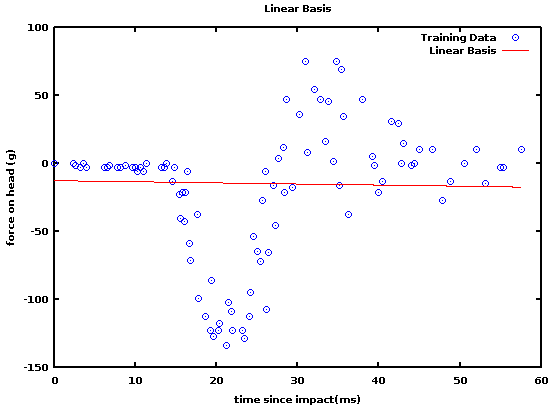
\includegraphics[scale=0.6]{gradient_descent}
  \caption{Warmup: Gradient Descent \label{gradientdescent}}
\end{figure}

As a baseline, we first a simple gradient descent. We also did a clearly overfit polynomial (using up to $n^12$).

\begin{figure}[h!] 
  \centering
  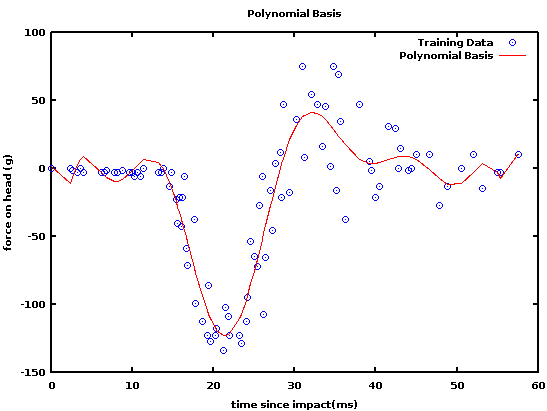
\includegraphics[scale=0.6]{polyfit}
  \caption{Warmup: Polynomial Fit $n^{12}$}
\end{figure}



\subsection*{Bayesian Linear Regression}

Using Moore Penrose, we solved for w.

\begin{figure}[h!] 
\centering
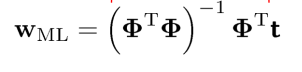
\includegraphics[scale=0.6]{moore_penrose}
\caption{Warmup: Moore Penrose (closed form)}
\end{figure}
 

\begin{figure}[h!] 
\centering
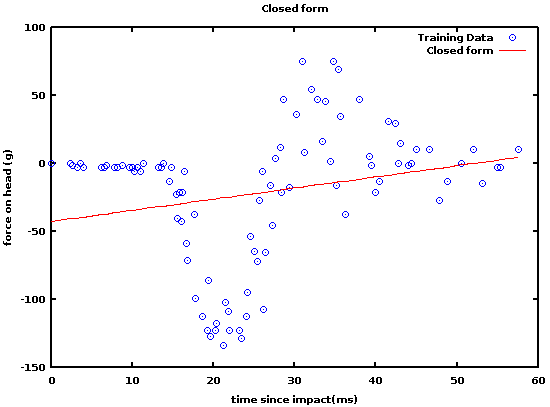
\includegraphics[scale=0.6]{closed_form}
\caption{Warmup: Gaussian (closed form)}
\end{figure}


\subsection*{Locally Weighted Linear Regression}

Locally weighted Linear Regression\footnote{Machine Learning in Action by Peter Harrington. \textsuperscript{\textcopyright} 2012 ISBN 978-1617290183} provided the lowest cost overall and a smooth fit to the data without overfitting given the profile of this dataset. A variety of $K$ values were attempted. 0.001 never converged. Values from 0.5, 1.0, 5.0 and 10.0 did converge with 1.0 seemingly providing the best balance between fit and smoothness.




\begin{figure}[h!] 
\centering
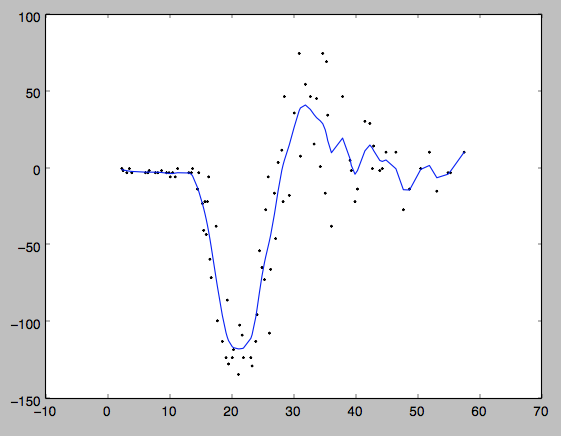
\includegraphics[scale=0.6]{lwlr}
\caption{Warmup: Locally Weighted Linear Regression}
\end{figure}

\begin{center}
    \begin{tabular}{| l | l |}
    \hline
    Method & Lowest Error \\ \hline
    Gradient Descent & 1293.0 \\
    Gaussian & 1187.7 \\
    Polynomial & 211.9 \\
    LWLR & 185.6 \\
    \hline
    \end{tabular}
\end{center}


\section*{Predicting Movie Opening Weekend Revenues}


\subsection*{Subsection 1}

\subsection*{Subsection 2}

\section*{Conclusion}


\end{document}  
